\documentclass[11pt,a4paper]{article}

% Package imports
\usepackage[utf8]{inputenc}
\usepackage[T1]{fontenc}
\usepackage{amsmath,amssymb,amsthm}
\usepackage{geometry}
\usepackage{booktabs}
\usepackage{tikz}
\usepackage{tikz-3dplot}
\usepackage{hyperref}
\usepackage{cleveref}
\usepackage{microtype}
\usepackage{breqn}  % For automatic equation breaking (dmath environment)

% Page geometry
\geometry{
  a4paper,
  margin=1in,
  marginparwidth=0.75in
}

% Hyperref setup
\hypersetup{
  colorlinks=true,
  linkcolor=blue,
  citecolor=blue,
  urlcolor=blue,
  pdfauthor={Feynkit Analysis},
  pdftitle={Triangle Graph Analysis}
}

% Better equation breaking
\allowdisplaybreaks

% Title and author
\title{Triangle Graph Analysis}
\author{Feynkit Analysis}
\date{\today}

\begin{document}

\maketitle

\begin{abstract}
This document presents a comprehensive analysis of a 1-loop Feynman integral with 3 internal propagators and 3 external legs. We compute the Symanzik polynomials, parametric representations, GKZ hypergeometric system, and toric ideal structure. All calculations were performed using Feynkit, a symbolic computation toolkit for Feynman integrals.
\end{abstract}

\tableofcontents
\clearpage

\section{Introduction}
\label{sec:introduction}

This report analyses the structure of a Feynman integral using modern algebraic geometry and differential equations techniques. We employ the parametric representation framework and study the integral through its associated GKZ $A$-hypergeometric system.

\section{Graph Properties}
\label{sec:graph}

We begin by describing the topological structure of the Feynman diagram.

\begin{figure}[htbp]
\centering
\begin{tikzpicture}[
  vertex/.style={circle, fill=black, inner sep=2pt},
  external/.style={circle, draw=black, inner sep=1.5pt},
  propagator/.style={thick},
  external_leg/.style={dashed}
]

  % Internal vertices
  \node[vertex] (v1) at (90:2cm) {};
  \node[vertex] (v2) at (210:2cm) {};
  \node[vertex] (v3) at (330:2cm) {};

  % Internal propagators
  \draw[propagator] (v1) -- (v2);
  \draw[propagator] (v2) -- (v3);
  \draw[propagator] (v3) -- (v1);

  % External legs
  \node[external] (e1) at (90.0:3.5cm) {};
  \draw[external_leg] (v1) -- (e1);
  \node[external] (e2) at (210.0:3.5cm) {};
  \draw[external_leg] (v2) -- (e2);
  \node[external] (e3) at (330.0:3.5cm) {};
  \draw[external_leg] (v3) -- (e3);

\end{tikzpicture}
\caption{Feynman diagram topology. Internal vertices are shown as filled circles, internal propagators as solid lines, and external legs as dashed lines.}
\label{fig:feynman_graph}
\end{figure}

\subsection{Topological Invariants}
\label{sec:topology}

The graph has the following topological properties, summarised in \Cref{tab:graph_properties}.

\begin{table}[htbp]
\centering
\begin{tabular}{@{}ll@{}}
\toprule
\textbf{Property} & \textbf{Value} \\
\midrule
Internal vertices & 3 \\
External legs & 3 \\
Internal propagators & 3 \\
Loop number & 1 \\
\bottomrule
\end{tabular}
\caption{Feynman graph topological properties.}
\label{tab:graph_properties}
\end{table}

\subsection{Edge Structure}
\label{sec:edges}

The complete list of edges is given in \Cref{tab:edges}.

\begin{table}[htbp]
\centering
\begin{tabular}{@{}ccccc@{}}
\toprule
\textbf{Index} & \textbf{Type} & \textbf{From} & \textbf{To} & \textbf{Mass} \\
\midrule
1 & Internal & 1 & 2 & $m_{1}$ \\
2 & Internal & 2 & 3 & $m_{2}$ \\
3 & Internal & 3 & 1 & $m_{3}$ \\
4 & External & 1 & 4 & --- \\
5 & External & 2 & 5 & --- \\
6 & External & 3 & 6 & --- \\
\bottomrule
\end{tabular}
\caption{Complete edge list for the Feynman graph.}
\label{tab:edges}
\end{table}

\clearpage
\section{Symanzik Polynomials}
\label{sec:symanzik}

The Symanzik polynomials $U$ and $F$ encode the topological and kinematic structure of the Feynman integral. These polynomials are fundamental to the parametric representation.

\subsection{First Symanzik Polynomial}
\label{sec:u_polynomial}

The first Symanzik polynomial $U$ depends only on the graph topology:
\begin{equation}
U = a_{1} + a_{2} + a_{3}
\label{eq:u_polynomial}
\end{equation}

This polynomial is homogeneous in the Schwinger parameters and encodes the sum over all spanning trees of the graph.

\subsection{Second Symanzik Polynomial}
\label{sec:f_polynomial}

The second Symanzik polynomial $F$ includes kinematic information:
\begin{dmath}
F = \frac{1}{\mu^{2}} \cdot \left(a_{1}^{2} \cdot m_{1}^{2} + a_{1} \cdot a_{2} \cdot m_{1}^{2} + a_{1} \cdot a_{2} \cdot m_{2}^{2} + \frac{s_{12}}{2} \cdot a_{1} \cdot a_{2} + \frac{s_{23}}{2} \cdot a_{1} \cdot a_{2} + a_{1} \cdot a_{3} \cdot m_{1}^{2} + a_{1} \cdot a_{3} \cdot m_{3}^{2} + \frac{s_{12}}{2} \cdot a_{1} \cdot a_{3} + \frac{s_{13}}{2} \cdot a_{1} \cdot a_{3} + a_{2}^{2} \cdot m_{2}^{2} + a_{2} \cdot a_{3} \cdot m_{2}^{2} + a_{2} \cdot a_{3} \cdot m_{3}^{2} + \frac{s_{13}}{2} \cdot a_{2} \cdot a_{3} + \frac{s_{23}}{2} \cdot a_{2} \cdot a_{3} + a_{3}^{2} \cdot m_{3}^{2}\right)
\label{eq:f_polynomial}
\end{dmath}

This polynomial encodes the momentum flow and mass structure of the diagram.

\clearpage
\section{Parametric Representations}
\label{sec:parametrisations}

We present three standard parametric representations: Schwinger, Feynman, and Lee-Pomeransky. Each representation has distinct advantages for different computational tasks.

\subsection{Schwinger Parametrisation}
\label{sec:schwinger}

Schwinger parametrisation with 3 alpha parameters. Each $\alpha \in [0, \infty)$. Integration domain is $\mathbb{R}_+^{3}$.

\paragraph{Parameters.}
The integration parameters are:
\begin{equation}
\alpha_{1}, \quad \alpha_{2}, \quad \alpha_{3}
\end{equation}

\paragraph{Prefactor.}
The overall prefactor is:
\begin{equation}
\frac{e^{\epsilon \cdot \gamma_{E}}}{\Gamma\left(\nu_{1}\right) \cdot \Gamma\left(\nu_{2}\right) \cdot \Gamma\left(\nu_{3}\right)}
\end{equation}

\paragraph{Measure.}
The integration measure is:
\begin{equation}
\alpha_{1}^{\nu_{1} - 1} \cdot \alpha_{2}^{\nu_{2} - 1} \cdot \alpha_{3}^{\nu_{3} - 1}
\end{equation}

\paragraph{Integrand.}
The integrand is:
\begin{dmath}
\left(\alpha_{1} + \alpha_{2} + \alpha_{3}\right)^{- \frac{D}{2}} \cdot e^{\frac{1}{2 \cdot \mu^{2} \cdot \left(\alpha_{1} + \alpha_{2} + \alpha_{3}\right)} \cdot \left(- 2 \cdot \alpha_{1}^{2} \cdot m_{1}^{2} - 2 \cdot \alpha_{1} \cdot \alpha_{2} \cdot m_{1}^{2} - 2 \cdot \alpha_{1} \cdot \alpha_{2} \cdot m_{2}^{2} - \alpha_{1} \cdot \alpha_{2} \cdot s_{12} - \alpha_{1} \cdot \alpha_{2} \cdot s_{23} - 2 \cdot \alpha_{1} \cdot \alpha_{3} \cdot m_{1}^{2} - 2 \cdot \alpha_{1} \cdot \alpha_{3} \cdot m_{3}^{2} - \alpha_{1} \cdot \alpha_{3} \cdot s_{12} - \alpha_{1} \cdot \alpha_{3} \cdot s_{13} - 2 \cdot \alpha_{2}^{2} \cdot m_{2}^{2} - 2 \cdot \alpha_{2} \cdot \alpha_{3} \cdot m_{2}^{2} - 2 \cdot \alpha_{2} \cdot \alpha_{3} \cdot m_{3}^{2} - \alpha_{2} \cdot \alpha_{3} \cdot s_{13} - \alpha_{2} \cdot \alpha_{3} \cdot s_{23} - 2 \cdot \alpha_{3}^{2} \cdot m_{3}^{2}\right)}
\end{dmath}

\subsection{Feynman Parametrisation}
\label{sec:feynman}

Feynman parametrisation with 3 parameters on the unit simplex. Constraint: $\sum_i a_i = 1$, all $a_i \geq 0$.

\paragraph{Parameters.}
The integration parameters are:
\begin{equation}
a_{1}, \quad a_{2}, \quad a_{3}
\end{equation}

\paragraph{Prefactor.}
The overall prefactor is:
\begin{equation}
\frac{e^{\epsilon \cdot \gamma_{E}}}{\Gamma\left(\nu_{1}\right) \cdot \Gamma\left(\nu_{2}\right) \cdot \Gamma\left(\nu_{3}\right)} \cdot \Gamma\left(- \frac{D}{2} + \nu_{1} + \nu_{2} + \nu_{3}\right)
\end{equation}

\paragraph{Measure.}
The integration measure is:
\begin{equation}
a_{1}^{\nu_{1} - 1} \cdot a_{2}^{\nu_{2} - 1} \cdot a_{3}^{\nu_{3} - 1}
\end{equation}

\paragraph{Integrand.}
The integrand is:
\begin{dmath}
\left(2 \cdot \mu^{2}\right)^{- \frac{D}{2} + \nu_{1} + \nu_{2} + \nu_{3}} \cdot \left(a_{1} + a_{2} + a_{3}\right)^{- D + \nu_{1} + \nu_{2} + \nu_{3}} \cdot \left(2 \cdot a_{1}^{2} \cdot m_{1}^{2} + 2 \cdot a_{1} \cdot a_{2} \cdot m_{1}^{2} + 2 \cdot a_{1} \cdot a_{2} \cdot m_{2}^{2} + a_{1} \cdot a_{2} \cdot s_{12} + a_{1} \cdot a_{2} \cdot s_{23} + 2 \cdot a_{1} \cdot a_{3} \cdot m_{1}^{2} + 2 \cdot a_{1} \cdot a_{3} \cdot m_{3}^{2} + a_{1} \cdot a_{3} \cdot s_{12} + a_{1} \cdot a_{3} \cdot s_{13} + 2 \cdot a_{2}^{2} \cdot m_{2}^{2} + 2 \cdot a_{2} \cdot a_{3} \cdot m_{2}^{2} + 2 \cdot a_{2} \cdot a_{3} \cdot m_{3}^{2} + a_{2} \cdot a_{3} \cdot s_{13} + a_{2} \cdot a_{3} \cdot s_{23} + 2 \cdot a_{3}^{2} \cdot m_{3}^{2}\right)^{\frac{D}{2} - \nu_{1} - \nu_{2} - \nu_{3}}
\end{dmath}

\paragraph{Constraints.}
The parameters satisfy the following constraints:
\begin{align}
a_{1} + a_{2} + a_{3} = 1
\end{align}

\subsection{Lee-Pomeransky Parametrisation}
\label{sec:lee_pomeransky}

Lee-Pomeransky parametrisation with 3 $u$ parameters. Each $u \in [0, \infty)$. Uses combined polynomial $G = U + F$. Integration domain is $\mathbb{R}_+^{3}$.

\paragraph{Parameters.}
The integration parameters are:
\begin{equation}
u_{1}, \quad u_{2}, \quad u_{3}
\end{equation}

\paragraph{Prefactor.}
The overall prefactor is:
\begin{equation}
\frac{e^{\epsilon \cdot \gamma_{E}} \cdot \Gamma\left(\frac{D}{2}\right)}{\Gamma\left(\nu_{1}\right) \cdot \Gamma\left(\nu_{2}\right) \cdot \Gamma\left(\nu_{3}\right) \cdot \Gamma\left(D - \nu_{1} - \nu_{2} - \nu_{3}\right)}
\end{equation}

\paragraph{Measure.}
The integration measure is:
\begin{equation}
u_{1}^{\nu_{1} - 1} \cdot u_{2}^{\nu_{2} - 1} \cdot u_{3}^{\nu_{3} - 1}
\end{equation}

\paragraph{Integrand.}
The integrand is:
\begin{dmath}
\left(\sqrt{2} \cdot \mu\right)^{D} \cdot \left(2 \cdot m_{1}^{2} \cdot u_{1}^{2} + 2 \cdot m_{1}^{2} \cdot u_{1} \cdot u_{2} + 2 \cdot m_{1}^{2} \cdot u_{1} \cdot u_{3} + 2 \cdot m_{2}^{2} \cdot u_{1} \cdot u_{2} + 2 \cdot m_{2}^{2} \cdot u_{2}^{2} + 2 \cdot m_{2}^{2} \cdot u_{2} \cdot u_{3} + 2 \cdot m_{3}^{2} \cdot u_{1} \cdot u_{3} + 2 \cdot m_{3}^{2} \cdot u_{2} \cdot u_{3} + 2 \cdot m_{3}^{2} \cdot u_{3}^{2} + 2 \cdot \mu^{2} \cdot \left(u_{1} + u_{2} + u_{3}\right) + s_{12} \cdot u_{1} \cdot u_{2} + s_{12} \cdot u_{1} \cdot u_{3} + s_{13} \cdot u_{1} \cdot u_{3} + s_{13} \cdot u_{2} \cdot u_{3} + s_{23} \cdot u_{1} \cdot u_{2} + s_{23} \cdot u_{2} \cdot u_{3}\right)^{- \frac{D}{2}}
\end{dmath}

\clearpage
\section{GKZ Hypergeometric System}
\label{sec:gkz}

The Feynman integral satisfies a system of partial differential equations known as the GKZ (Gelfand-Kapranov-Zelevinsky) $A$-hypergeometric system. This system provides a systematic approach to studying the analytic properties of the integral.

\subsection{GKZ $A$-Hypergeometric System}
\label{sec:gkz_system}

The GKZ hypergeometric system has 9 variables, 4 differential equations, and A-matrix of dimension $4 \times 9$.

\paragraph{$A$-matrix.}
The $A$-matrix encoding the monomial exponent structure is:
\begin{equation}
A = \left[\begin{matrix}1 & 1 & 1 & 1 & 1 & 1 & 1 & 1 & 1\\2 & 1 & 1 & 1 & 0 & 0 & 0 & 0 & 0\\0 & 1 & 0 & 0 & 2 & 1 & 1 & 0 & 0\\0 & 0 & 1 & 0 & 0 & 1 & 0 & 2 & 1\end{matrix}\right]
\label{eq:a_matrix}
\end{equation}

\paragraph{Newton polytope.}
The Newton polytope is the convex hull of the monomial support.
It encodes the combinatorial structure of the polynomial $G(u) = U(u) + F(u)$.
The polytope is visualised in \Cref{fig:newton_polytope}.

\begin{figure}[htbp]
\centering
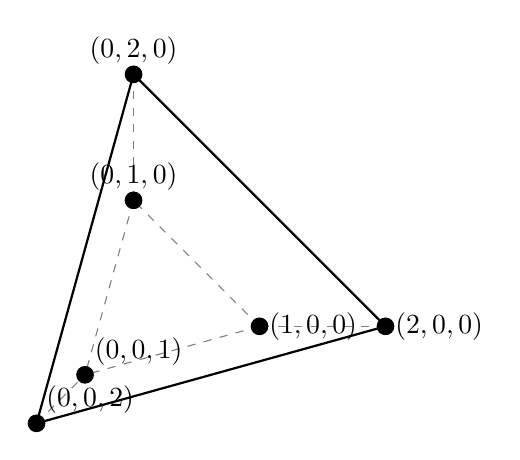
\begin{tikzpicture}[scale=1.6]
    % Newton Polytope

    % Hidden edges (behind the polytope)
    \draw[dashed,gray] (1.0,0.0,0.0) -- (0.0,0.0,1.0);
    \draw[dashed,gray] (0.0,1.0,0.0) -- (0.0,0.0,1.0);
    \draw[dashed,gray] (0.0,2.0,0.0) -- (0.0,1.0,0.0);
    \draw[dashed,gray] (2.0,0.0,0.0) -- (1.0,0.0,0.0);
    \draw[dashed,gray] (1.0,0.0,0.0) -- (0.0,1.0,0.0);
    \draw[dashed,gray] (0.0,0.0,2.0) -- (0.0,0.0,1.0);

    % Visible edges (in front)
    \draw[thick,black] (2.0,0.0,0.0) -- (0.0,0.0,2.0);
    \draw[thick,black] (2.0,0.0,0.0) -- (0.0,2.0,0.0);
    \draw[thick,black] (0.0,2.0,0.0) -- (0.0,0.0,2.0);

    % Vertex labels
    \fill (2.0,0.0,0.0) circle (2pt);
    \node[right] at (2.0,0.0,0.0) {$(2,0,0)$};
    \fill (1.0,0.0,0.0) circle (2pt);
    \node[right] at (1.0,0.0,0.0) {$(1,0,0)$};
    \fill (0.0,2.0,0.0) circle (2pt);
    \node[above] at (0.0,2.0,0.0) {$(0,2,0)$};
    \fill (0.0,1.0,0.0) circle (2pt);
    \node[above] at (0.0,1.0,0.0) {$(0,1,0)$};
    \fill (0.0,0.0,2.0) circle (2pt);
    \node[above right] at (0.0,0.0,2.0) {$(0,0,2)$};
    \fill (0.0,0.0,1.0) circle (2pt);
    \node[above right] at (0.0,0.0,1.0) {$(0,0,1)$};
\end{tikzpicture}
\caption{Newton polytope of the Lee-Pomeransky polynomial $G(u) = U(u) + F(u)$. Vertices represent monomial exponent vectors, solid edges are visible from the viewing angle, and dashed edges are hidden behind faces.}
\label{fig:newton_polytope}
\end{figure}

\paragraph{Parameter vector.}
The parameter vector $\boldsymbol{\beta}$ is:
\begin{equation}
\boldsymbol{\beta} = \begin{pmatrix}
- \frac{D}{2} + \nu_{1} + \nu_{2} + \nu_{3} \\
\nu_{1} \\
\nu_{2} \\
\nu_{3}
\end{pmatrix}
\label{eq:beta_vector}
\end{equation}

\paragraph{Euler equations.}
The system consists of 4 Euler-type differential equations. These are Horn-type hypergeometric differential equations, where $\Phi = \Phi(z_1, \ldots, z_{9})$ represents the Feynman integral.
Each equation has the form:
\begin{dmath}
z_{1} \cdot \frac{\partial}{\partial z_{1}} \Phi + z_{2} \cdot \frac{\partial}{\partial z_{2}} \Phi + z_{3} \cdot \frac{\partial}{\partial z_{3}} \Phi + z_{4} \cdot \frac{\partial}{\partial z_{4}} \Phi + z_{5} \cdot \frac{\partial}{\partial z_{5}} \Phi + z_{6} \cdot \frac{\partial}{\partial z_{6}} \Phi + z_{7} \cdot \frac{\partial}{\partial z_{7}} \Phi + z_{8} \cdot \frac{\partial}{\partial z_{8}} \Phi + z_{9} \cdot \frac{\partial}{\partial z_{9}} \Phi = \left(- \frac{D}{2} + \nu_{1} + \nu_{2} + \nu_{3}\right) \cdot \Phi
\label{eq:euler_0}
\end{dmath}
\begin{dmath}
2 \cdot z_{1} \cdot \frac{\partial}{\partial z_{1}} \Phi + z_{2} \cdot \frac{\partial}{\partial z_{2}} \Phi + z_{3} \cdot \frac{\partial}{\partial z_{3}} \Phi + z_{4} \cdot \frac{\partial}{\partial z_{4}} \Phi = \nu_{1} \cdot \Phi
\label{eq:euler_1}
\end{dmath}
\begin{dmath}
z_{2} \cdot \frac{\partial}{\partial z_{2}} \Phi + 2 \cdot z_{5} \cdot \frac{\partial}{\partial z_{5}} \Phi + z_{6} \cdot \frac{\partial}{\partial z_{6}} \Phi + z_{7} \cdot \frac{\partial}{\partial z_{7}} \Phi = \nu_{2} \cdot \Phi
\label{eq:euler_2}
\end{dmath}
\begin{dmath}
z_{3} \cdot \frac{\partial}{\partial z_{3}} \Phi + z_{6} \cdot \frac{\partial}{\partial z_{6}} \Phi + 2 \cdot z_{8} \cdot \frac{\partial}{\partial z_{8}} \Phi + z_{9} \cdot \frac{\partial}{\partial z_{9}} \Phi = \nu_{3} \cdot \Phi
\label{eq:euler_3}
\end{dmath}

Each equation expresses a homogeneity property of the Feynman integral under rescalings of the Lee-Pomeransky parameters.

\clearpage
\section{Algebraic Structure}
\label{sec:algebra}

\subsection{Toric Ideal and Integration-by-Parts Relations}
\label{sec:toric_ideal}

The toric ideal $I_A$ is generated by 14 polynomials.
These generators encode integration-by-parts (IBP) relations among the
monomial coefficients of the Lee-Pomeransky polynomial.

\paragraph{Generators.}
The toric ideal is generated by:
\begin{equation}
z_{1} \cdot z_{5} - z_{2}^{2} = 0
\label{eq:toric_gen_0}
\end{equation}
\begin{equation}
z_{1} \cdot z_{6} - z_{2} \cdot z_{3} = 0
\label{eq:toric_gen_1}
\end{equation}
\begin{equation}
z_{1} \cdot z_{7} - z_{2} \cdot z_{4} = 0
\label{eq:toric_gen_2}
\end{equation}
\begin{equation}
z_{1} \cdot z_{8} - z_{3}^{2} = 0
\label{eq:toric_gen_3}
\end{equation}
\begin{equation}
z_{1} \cdot z_{9} - z_{3} \cdot z_{4} = 0
\label{eq:toric_gen_4}
\end{equation}
\begin{equation}
z_{2} \cdot z_{6} - z_{3} \cdot z_{5} = 0
\label{eq:toric_gen_5}
\end{equation}
\begin{equation}
z_{2} \cdot z_{7} - z_{4} \cdot z_{5} = 0
\label{eq:toric_gen_6}
\end{equation}
\begin{equation}
z_{2} \cdot z_{8} - z_{3} \cdot z_{6} = 0
\label{eq:toric_gen_7}
\end{equation}
\begin{equation}
z_{2} \cdot z_{9} - z_{4} \cdot z_{6} = 0
\label{eq:toric_gen_8}
\end{equation}
\begin{equation}
z_{3} \cdot z_{7} - z_{4} \cdot z_{6} = 0
\label{eq:toric_gen_9}
\end{equation}
\begin{equation}
z_{3} \cdot z_{9} - z_{4} \cdot z_{8} = 0
\label{eq:toric_gen_10}
\end{equation}
\begin{equation}
z_{5} \cdot z_{8} - z_{6}^{2} = 0
\label{eq:toric_gen_11}
\end{equation}
\begin{equation}
z_{5} \cdot z_{9} - z_{6} \cdot z_{7} = 0
\label{eq:toric_gen_12}
\end{equation}
\begin{equation}
z_{6} \cdot z_{9} - z_{7} \cdot z_{8} = 0
\label{eq:toric_gen_13}
\end{equation}

Each generator represents a syzygy (polynomial relation) among the monomials,
which corresponds to an IBP reduction identity for the Feynman integral.
These relations can be used to express the integral in terms of simpler master integrals.

\section{Conclusion}
\label{sec:conclusion}

This analysis provides a complete mathematical characterisation of the Feynman integral. The parametric representations enable systematic evaluation, while the GKZ system and toric ideal structure reveal the underlying algebraic-geometric properties.

\appendix

\section{Computational Details}
\label{sec:computational}

All calculations in this document were performed using Feynkit, a Python package for symbolic Feynman integral computations. The source code is available at \texttt{https://github.com/feynkit/feynkit}.

\end{document}
